\section{The IAU Solar System Body Centered Orientation } \label{sec:gendet} 
This section is an elaboration of the basic IAU system defined in Section 2.
Planetary coordinate systems are defined relative to their mean axis of rotation and various definitions of longitude depending on the body. The longitude systems of most of those bodies with observable rigid surfaces have been defined by references to a surface feature such as a crater. Approximate expressions for these rotational elements with respect to the ICRF have been derived. 
The north pole is that pole of rotation that lies on the north side of the invariable plane of the solar system. The direction of the north pole is specified by the value of its right ascension $\alpha_0$ and declination $\delta_0$. With the pole so specified, the two intersection points of the body's equator and the ICRF equator are $\alpha_0$ +90, define it as the node Q. Suppose the prime meridian has been chosen so that it crosses the body's equator at point B. Then specify the location of the prime meridian by providing a value for W, the angle measured easterly along the body's equator between the node the first sign of Aries $\aries$ and the intersection of the body equator and the ICRF equator (see Fig. 3). The right ascension of the point is 90. + $\alpha_0$ and the inclination of the planet's equator to the celestial equator is 90-$\alpha_0$. As long as the planet, and hence its prime meridian, rotates uniformly,W varies nearly linearly with time. In addition, $\alpha_0$, $\delta_0$, and W may vary with time due to a precession of the axis of rotation of the body (or satellite). If W increases with time, the body has a direct (or prograde) rotation, and, if W decreases with time, the rotation is said to be retrograde.
Bodies without solid surfaces are very irregular solid surfaces, all have a prime meridian but have to be chosen in different ways , see the IAU publication \cite{IAU2006}.

\textbf{Coordinate Frame: } Rotating

\begin{itemize}
\item X - axis: Out the prime meridian.
\item Y - axis: Completes the right-handed system.
\item Z - axis: Defined as the pole vector of the body of interest, with epoch J2000 (where J2000 = Julian date 2451545.0 TDB (Barycentric Dynamical Time)). 
\end{itemize}
The north pole is that pole of rotation lies on the north side of the invariable plane of the solar system.

\begin{figure}[htp]
\centering
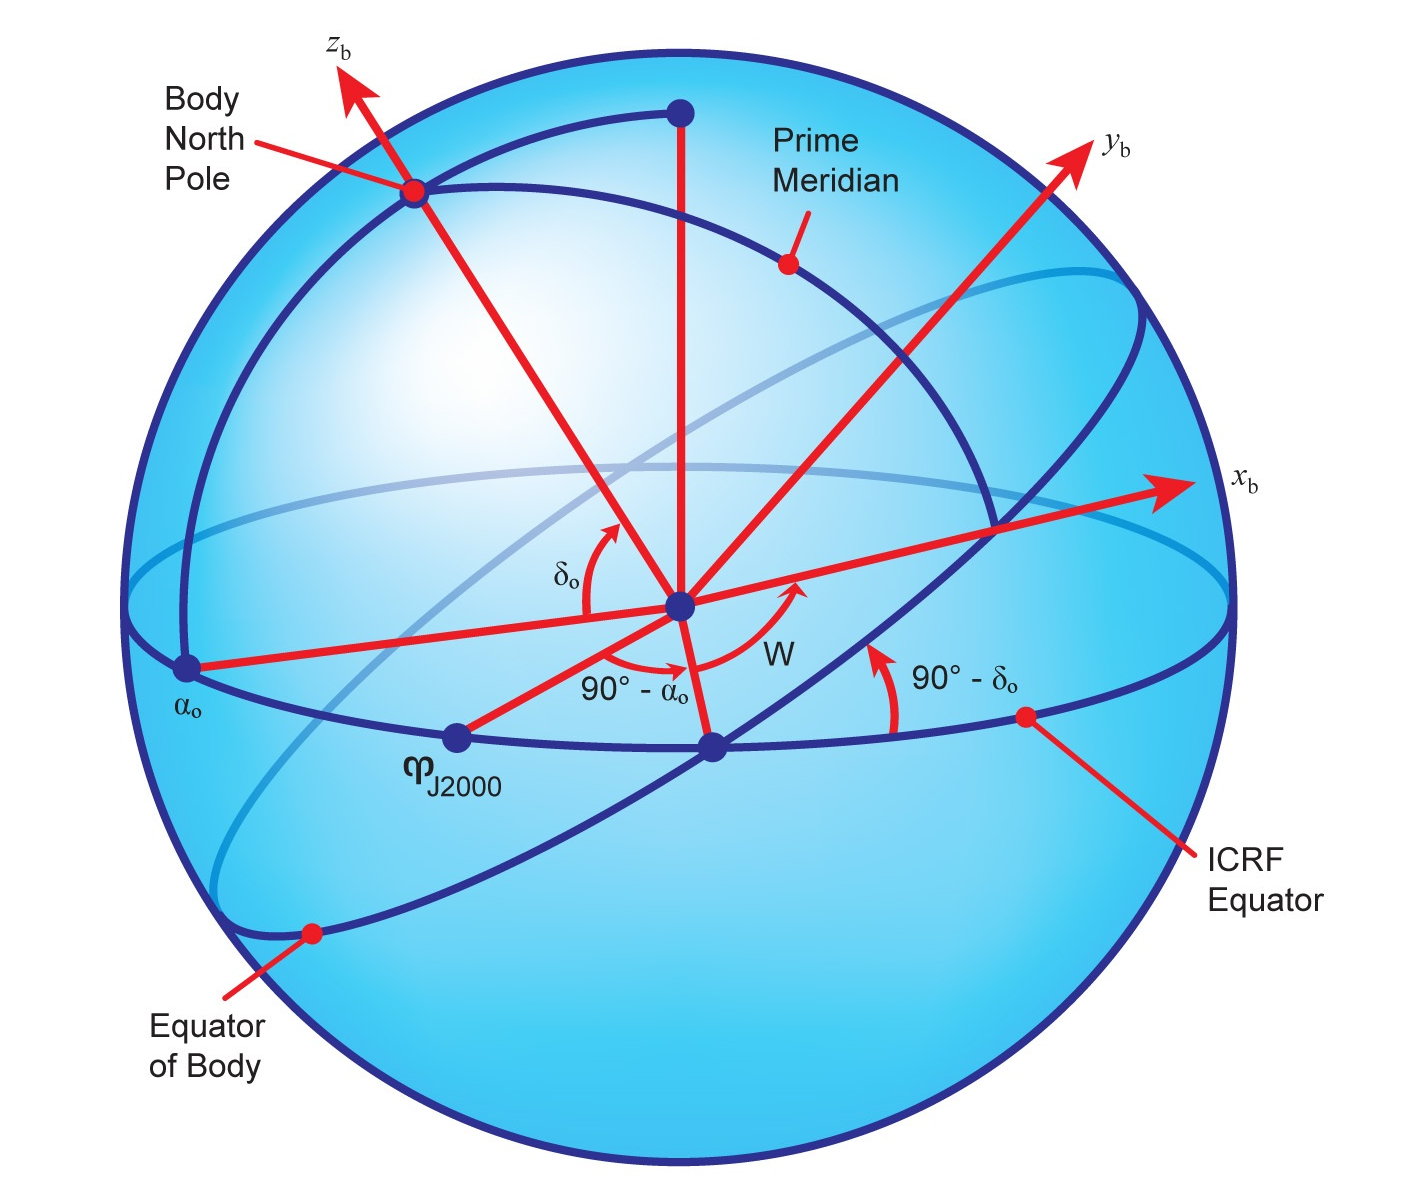
\includegraphics [width=7in]{figs/fig3.png}
\caption{Realization of the IAU Fixed Body Reference System}
\label{fig:3}
\end{figure}

\newpage
\subsection{Example IAU Body Centered}

The following rotation is used by the Planetary Data System (PDS) to transform 
from ICRF inertial to body fixed. The IAU specifies a simple formulation for $\alpha$,
$\beta$, , W and the rates of change of these parametes ,these can be either constands or a
and expansion in a periodic series \cite{IAU2006}.
The PDS rotation matric R is:

\begin{center}
$
R = R_1 ( - W)R_3 (\delta _0  - 90^ \circ)R_1 (\alpha _0  + 90^ \circ  )
$
\end{center}
where
\begin{center}
    \begin{equation}\nonumber
    R_1= \left[
    \begin{array}{rrr}
     1   & 0 &  0\\
     0 &  \cos(x)  & \sin(x) \\
     0 & -\sin(x) & \cos(x) 0   \\
    \end{array}\right]
    \end{equation}
\end{center}
and
\begin{center}
    \begin{equation}\nonumber
    R_3= \left[
    \begin{array}{rrr} 
     \cos(x)  & \sin(x) & 0\\
     -\sin(x) & \cos(x) & 0 \\
      0 & 0 & 1\\
     
    \end{array}\right]
    \end{equation}
\end{center}
and

One should consult the data sets at the PDS,
the web site at:
\begin{verbatim}
http://pds.nasa.gov/
\end{verbatim}

As noted in Section 2 more elaborate body orientations apply to the Earth and Moon because of their modeled non-spherical fields. Other bodies may be modeled this way too.


